% CVPR camera-ready style report draft.
% Copy this file into the official CVPR LaTeX template folder together with references.bib.
% IMPORTANT: keep camera-ready mode for the final submission: use \usepackage{cvpr}, not \usepackage[review]{cvpr}.

\documentclass[10pt,twocolumn,letterpaper]{article}

\usepackage{cvpr}
\usepackage{times}
\usepackage{epsfig}
\usepackage{graphicx}
\usepackage{amsmath}
\usepackage{amssymb}
\usepackage{booktabs}
\usepackage{multirow}
\usepackage{array}
\usepackage{xcolor}
\usepackage{url}

\definecolor{cvprblue}{rgb}{0.21,0.49,0.74}
\usepackage[pagebackref,breaklinks,colorlinks,citecolor=cvprblue,linkcolor=cvprblue,urlcolor=cvprblue]{hyperref}

\def\paperID{0000}
\def\confName{CVPR}
\def\confYear{2026}

\title{Practical Video Super-Resolution with Classical Baselines, Real-ESRGAN, BasicVSR, and Temporal Refinement}

\author{Junyi He \\
Binkai Liu \\
Introduction to Computer Vision \\
}

\begin{document}
\maketitle

\begin{abstract}
Video super-resolution (VSR) aims to recover high-resolution, temporally coherent videos from low-resolution inputs. This project implements and evaluates a complete three-part VSR pipeline. First, we build reproducible baselines using bicubic and Lanczos interpolation, a lightweight SRCNN-style model, temporal averaging, and unsharp masking. Second, we reproduce stronger pretrained methods, including Real-ESRGAN for perceptual frame restoration and BasicVSR for video-based feature propagation. Third, we explore refinement strategies for the remaining failure cases, including optical-flow temporal stabilization, uncertainty-aware adaptive fusion, rectified-flow/diffusion-style refinement, and a distilled streaming diffusion direction. Experiments on the mandatory REDS-sample, Vimeo-LR, and wild videos show that Real-ESRGAN is the strongest practical visual baseline, while optical-flow stabilization improves temporal behavior without expensive retraining. On a 20-clip Vimeo-90K subset with ground truth, flow-stabilized Real-ESRGAN improves Real-ESRGAN from 25.0214 to 25.2300 PSNR, from 0.7895 to 0.7949 SSIM, and from 0.1611 to 0.1593 LPIPS. Code and results are available at: \textbf{\url{https://github.com/Junyi-111/Video-Super-Resolution.git}}
\end{abstract}

\section{Introduction}

Video super-resolution reconstructs high-resolution (HR) videos from low-resolution (LR) inputs. Unlike single-image super-resolution, VSR must balance two goals at the same time: each frame should contain sharp and plausible spatial details, and adjacent frames should remain temporally stable. A frame-wise method can improve apparent sharpness while still producing flicker, texture popping, or hallucinated details that change from frame to frame.

This project follows the course roadmap and implements three stages. Part 1 establishes classical and lightweight learning baselines. Part 2 applies modern pretrained methods, focusing on Real-ESRGAN~\cite{wang2021realesrgan} and BasicVSR~\cite{chan2021basicvsr}. Part 3 studies practical extensions for the limitations observed in Part 2, especially temporal inconsistency and generative artifacts. We also evaluate an optional 20-clip Vimeo-90K~\cite{xue2019vimeo90k} subset with ground-truth HR frames to provide a standard benchmark beyond the mandatory data.

Our main finding is that the best method depends on the evaluation target. Bicubic interpolation can score highly on PSNR and SSIM under mild, pixel-aligned synthetic degradation, but it remains visually blurry. Real-ESRGAN produces sharper perceptual detail and much better LPIPS. Optical-flow stabilization slightly improves Real-ESRGAN on the Vimeo-90K subset and is the most reliable Part 3 refinement. Diffusion-style and distilled streaming methods are promising, but they require careful control because they can introduce hallucinated details and temporal instability.

\section{Related Work}

\noindent\textbf{Classical and CNN image super-resolution.}
Interpolation methods such as bicubic and Lanczos are fast and deterministic, but they cannot synthesize missing high-frequency details. SRCNN~\cite{dong2015srcnn} was an early convolutional approach that learned the LR-to-HR mapping directly from data. SRGAN~\cite{ledig2017srgan} introduced adversarial and perceptual losses to improve photo-realistic texture, while EDSR~\cite{lim2017edsr} improved residual network design for high-fidelity single-image super-resolution.

\noindent\textbf{Video super-resolution and alignment.}
VSR methods exploit temporal redundancy across neighboring frames. EDVR~\cite{wang2019edvr} uses enhanced deformable convolutions for video restoration. TDAN~\cite{tian2020tdan} performs temporally deformable alignment. BasicVSR~\cite{chan2021basicvsr} shows that bidirectional propagation, optical flow alignment, and recurrent hidden states are essential components for efficient VSR. BasicVSR++~\cite{chan2022basicvsrpp} further improves propagation and alignment with second-order grid propagation and flow-guided deformable alignment.

\noindent\textbf{Generative and perceptual restoration.}
Real-ESRGAN~\cite{wang2021realesrgan} trains on synthetic degradations for real-world blind super-resolution and is robust for arbitrary videos. SR3~\cite{saharia2022sr3} demonstrates iterative refinement with diffusion models for image super-resolution. Flow Matching~\cite{lipman2023flowmatching} provides a generative modeling framework with straighter probability-flow trajectories. ControlNet~\cite{zhang2023controlnet} adds conditional control to diffusion models, and latent diffusion models~\cite{rombach2022ldm} provide efficient high-resolution image synthesis. LoRA~\cite{hu2022lora} is relevant as a lightweight adaptation method for large generative models.

\noindent\textbf{Datasets and metrics.}
REDS~\cite{nah2019reds} and Vimeo-90K~\cite{xue2019vimeo90k} are widely used video restoration datasets. We report PSNR, SSIM~\cite{wang2004ssim}, LPIPS~\cite{zhang2018lpips}, temporal MAE, and a temporal LPIPS-style proxy inspired by temporally coherent video synthesis work~\cite{chu2020tgan}.

\section{Method}

Figure~\ref{fig:pipeline} summarizes the complete project pipeline.

\begin{figure*}[t]
    \centering
    % FIGURE: generated by scripts/make_report_assets.py.
    % Existing path in this repository: output/figures/report_pipeline_flowchart.png
    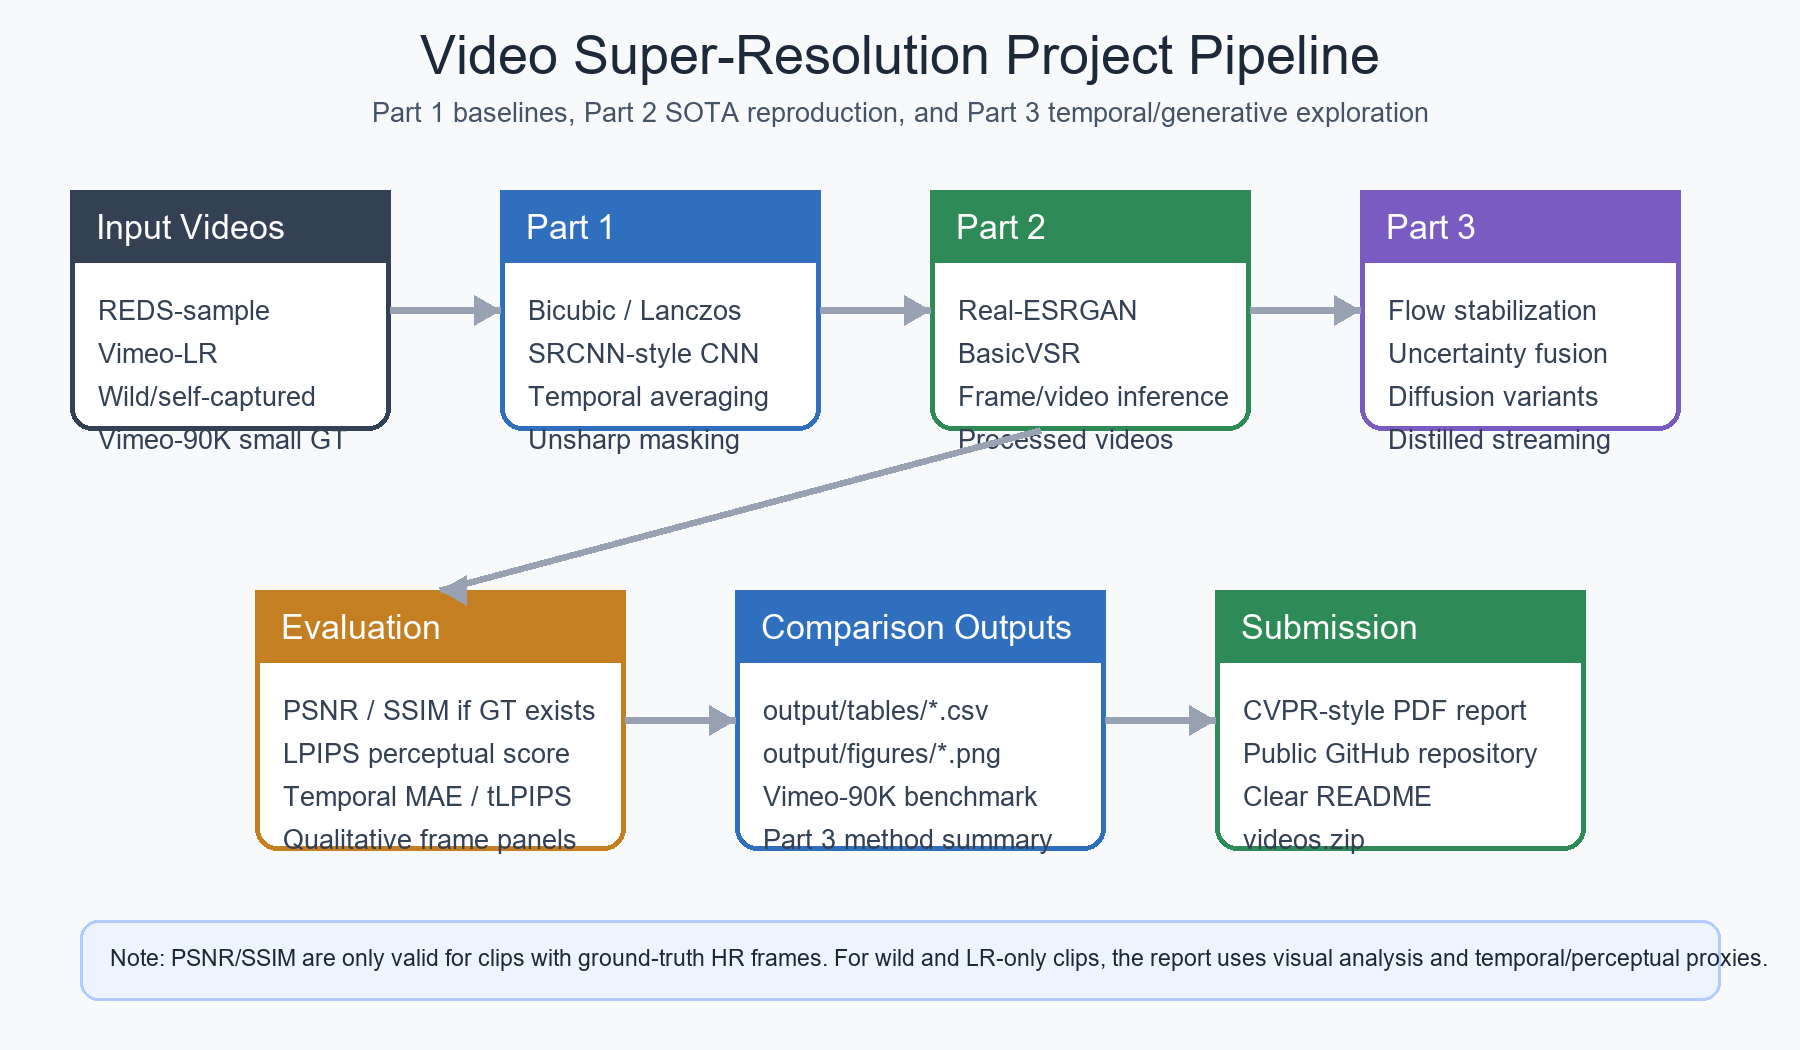
\includegraphics[width=0.96\textwidth]{../../output/figures/report_pipeline_flowchart.png}
    \caption{Overall pipeline. Part 1 builds classical and lightweight baselines, Part 2 applies Real-ESRGAN and BasicVSR, and Part 3 explores temporal and generative refinements. Full-reference metrics are used only when ground-truth HR frames are available.}
    \label{fig:pipeline}
\end{figure*}

\subsection{Part 1: Baseline Pipeline}

The baseline stage is designed to make the data flow reproducible before applying heavy models. For each input video, we decode frames, apply spatial upsampling, optionally apply a lightweight temporal operation, and re-encode the processed frames into videos. Bicubic and Lanczos interpolation are used as absolute baselines. We also implement a compact SRCNN-style model following the three-layer CNN idea in~\cite{dong2015srcnn}. Finally, we test temporal averaging and unsharp masking to observe the trade-off between denoising, blur, and edge enhancement.

These baselines are not expected to recover complex textures. Their role is to verify frame order, scale factor, video I/O, and metric computation. They also provide a fair lower bound for comparing stronger methods.

\subsection{Part 2: SOTA Reproduction}

Part 2 evaluates two stronger methods. Real-ESRGAN is applied frame by frame. This ignores long-range temporal structure, but it is robust on real-world degradations and produces strong perceptual sharpness. BasicVSR is a video model that propagates features bidirectionally and uses optical flow for alignment. In principle, BasicVSR should improve temporal consistency by aggregating neighboring frames. In our experiments, however, Real-ESRGAN was more visually reliable on the mixed mandatory data. BasicVSR was sensitive to the gap between the pretrained degradation setting and our real or synthetically degraded clips.

\subsection{Part 3: Exploration and Refinement}

Part 3 studies the limitations of direct inference. We evaluated four directions.

\noindent\textbf{Direction A: rectified-flow/diffusion-style refinement.}
This direction tests whether generative refinement can restore high-frequency textures beyond deterministic VSR outputs. It is motivated by SR3 and Flow Matching. In practice, we observed that generative refinement can improve local texture but may alter content or create inconsistent details.

\noindent\textbf{Direction B: optical-flow temporal stabilization.}
This direction is our most practical final refinement. Given a Real-ESRGAN output sequence, we estimate motion between neighboring frames and use optical-flow-guided blending to reduce flicker. This method is lightweight, does not require training, and directly targets frame-wise instability.

\noindent\textbf{Direction C: uncertainty-aware adaptive fusion.}
This direction follows the idea that different regions need different restoration behavior. Reliable structures such as edges, faces, and text should remain conservative, while uncertain textures such as grass or water may benefit from generative enhancement. We approximate pixel-wise uncertainty with local disagreement and confidence cues, then adaptively blend conservative and enhanced candidates. The idea is strong, but the current implementation did not consistently outperform the simpler flow-stabilized pipeline.

\noindent\textbf{Direction D: distilled streaming diffusion.}
A teammate implemented an additional distilled streaming direction, partly motivated by efficient attention and streaming generative restoration. It achieved promising PSNR, SSIM, and LPIPS in the current Part 3 table, but its temporal MAE is worse than some alternatives. We therefore report it as an exploratory result rather than our most stable final recommendation.

\section{Experiments}

\subsection{Datasets}

We evaluate on the mandatory course data and an optional benchmark subset:

\begin{itemize}
    \item \textbf{Wild video:} self-captured low-resolution video for real-world generalization.
    \item \textbf{Provided sample data:} REDS-sample and Vimeo-LR clips.
    \item \textbf{Standard benchmark:} a 20-clip Vimeo-90K subset with HR ground truth.
\end{itemize}

For LR-only videos without HR ground truth, PSNR and SSIM are not valid. We therefore use qualitative comparison and temporal/perceptual proxy metrics for those videos. For the Vimeo-90K subset, ground truth is available, so we report PSNR, SSIM, LPIPS, and temporal MAE.

\subsection{Metrics}

PSNR and SSIM measure full-reference pixel and structural fidelity. LPIPS measures perceptual similarity using deep features. Temporal MAE measures the average frame-to-frame difference and is used as a simple temporal stability proxy. We also report tLPIPS-style values for Part 3 comparisons when available. Lower LPIPS, temporal MAE, and tLPIPS indicate better perceptual or temporal consistency.

\subsection{Vimeo-90K Small Benchmark}

Table~\ref{tab:vimeo} reports the 20-clip Vimeo-90K subset. Bicubic has the best PSNR and SSIM because the benchmark degradation is mild and pixel-aligned, so conservative reconstruction is rewarded. However, Real-ESRGAN greatly improves LPIPS, indicating better perceptual quality. Flow-stabilized Real-ESRGAN improves Real-ESRGAN across all four reported metrics, making it the best practical learned/perceptual method in this subset.

\begin{table}[t]
\centering
\caption{Vimeo-90K small benchmark on 20 clips. Higher PSNR/SSIM is better; lower LPIPS/Temporal MAE is better.}
\label{tab:vimeo}
\resizebox{\linewidth}{!}{%
\begin{tabular}{lccccc}
\toprule
Method & Clips & PSNR $\uparrow$ & SSIM $\uparrow$ & LPIPS $\downarrow$ & Temp. MAE $\downarrow$ \\
\midrule
Bicubic & 20 & \textbf{27.1938} & \textbf{0.8315} & 0.3082 & \textbf{10.7551} \\
Real-ESRGAN & 20 & 25.0214 & 0.7895 & 0.1611 & 11.2486 \\
BasicVSR & 20 & 23.1032 & 0.7643 & 0.2197 & 16.4366 \\
Flow-Stabilized & 20 & 25.2300 & 0.7949 & \textbf{0.1593} & 10.8161 \\
\bottomrule
\end{tabular}}
\end{table}

\begin{figure}[t]
    \centering
    % FIGURE: keep this if the file exists, otherwise replace with your own Vimeo-90K panel.
    % Existing path: output/figures/vimeo90k_small/vimeo90k_00001_0389_frame2_panel.png
    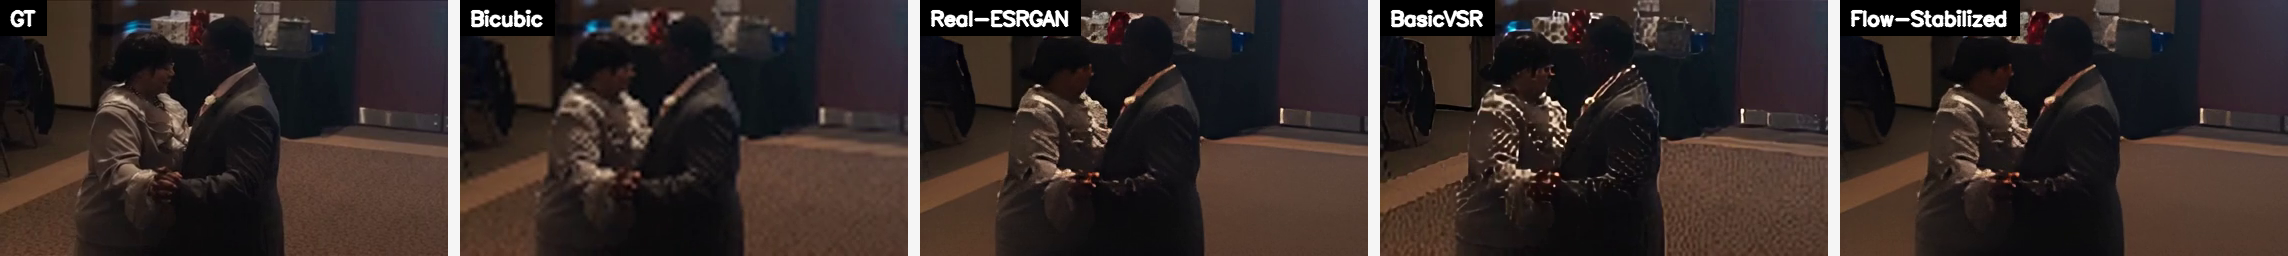
\includegraphics[width=\linewidth]{../../output/figures/vimeo90k_small/vimeo90k_00001_0389_frame2_panel.png}
    \caption{Qualitative Vimeo-90K comparison. Replace or crop this panel manually if you want larger zoomed patches in the final PDF.}
    \label{fig:vimeo_panel}
\end{figure}

\subsection{Part 3 Comparison}

Table~\ref{tab:part3} compares the Part 3 exploratory methods. Direction D obtains the best PSNR, SSIM, and LPIPS in this table, while the temporal Real-ESRGAN blend gives the lowest temporal MAE. Direction B remains the most stable final recommendation because it is reproducible and directly addresses flicker without requiring a large generative dependency stack.

\begin{table}[t]
\centering
\caption{Part 3 exploratory comparison on the available evaluated sequence. Higher PSNR/SSIM is better; lower LPIPS/tLPIPS/Temporal MAE is better.}
\label{tab:part3}
\resizebox{\linewidth}{!}{%
\begin{tabular}{lccccc}
\toprule
Method & PSNR $\uparrow$ & SSIM $\uparrow$ & LPIPS $\downarrow$ & tLPIPS $\downarrow$ & Temp. MAE $\downarrow$ \\
\midrule
Rectified-flow & 13.9390 & 0.8184 & 0.1453 & 0.0948 & 6.4678 \\
Flow-stabilized & 13.9781 & 0.8204 & 0.1439 & 0.0953 & 6.3549 \\
Temporal + Real-ESRGAN blend & 13.8252 & 0.8141 & 0.1638 & 0.1229 & \textbf{5.6631} \\
Uncertainty-adaptive & 13.9199 & 0.8169 & 0.1436 & \textbf{0.0921} & 6.4898 \\
Streaming distilled diffusion & \textbf{14.0615} & \textbf{0.8250} & \textbf{0.1344} & 0.1022 & 7.4867 \\
\bottomrule
\end{tabular}}
\end{table}

\section{Qualitative Analysis}

Figure~\ref{fig:wild_part2} compares Real-ESRGAN and BasicVSR on the wild video. Real-ESRGAN tends to produce sharper local edges and stronger texture enhancement. BasicVSR is designed for temporal propagation, but in our current setting it can look softer and may not match Real-ESRGAN's perceptual detail.

\begin{figure}[t]
    \centering
    % FIGURE: existing wild Real-ESRGAN vs BasicVSR full-frame panel.
    % Existing path: output/figures/wild_realesrgan_basicvsr/wild_frame_0080_full.png
    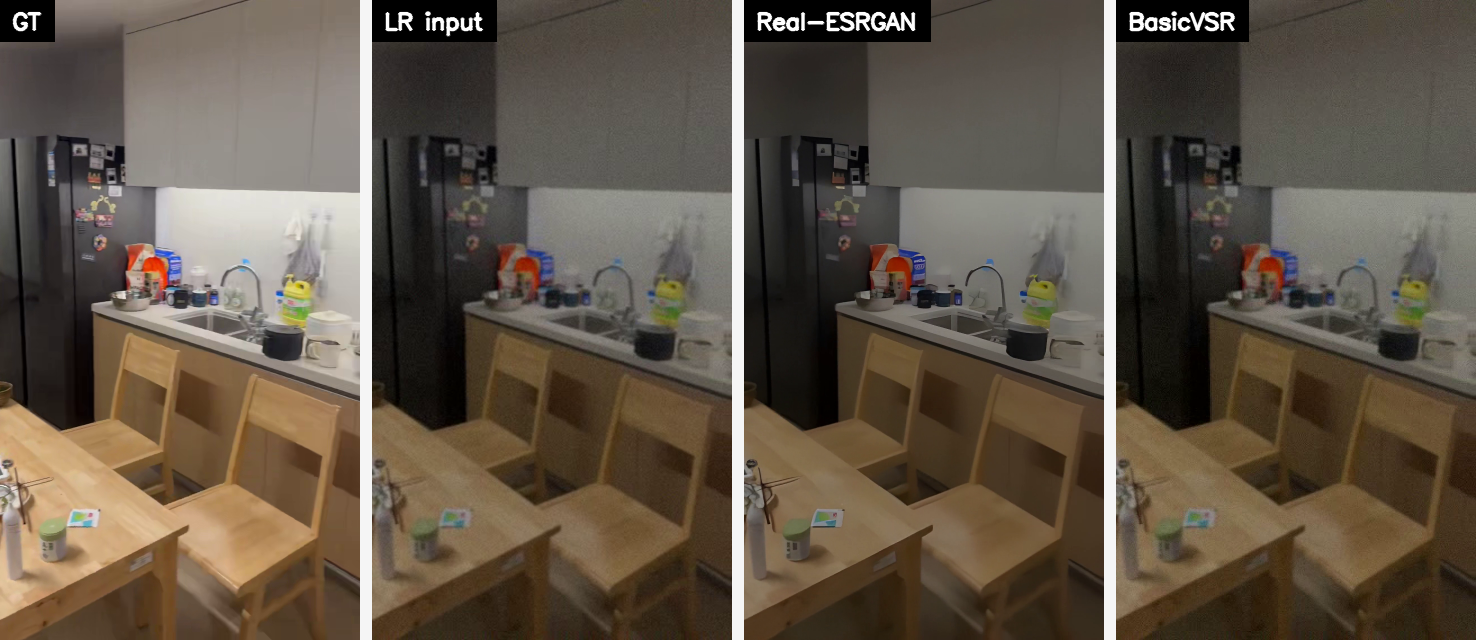
\includegraphics[width=\linewidth]{../../output/figures/wild_realesrgan_basicvsr/wild_frame_0080_full.png}
    \caption{Wild-video qualitative comparison between Real-ESRGAN and BasicVSR. Manually replace with a sharper crop if needed.}
    \label{fig:wild_part2}
\end{figure}

\begin{figure}[t]
    \centering
    % FIGURE: existing zoom panel for local detail comparison.
    % Existing path: output/figures/wild_realesrgan_basicvsr/wild_frame_0080_zoom.png
    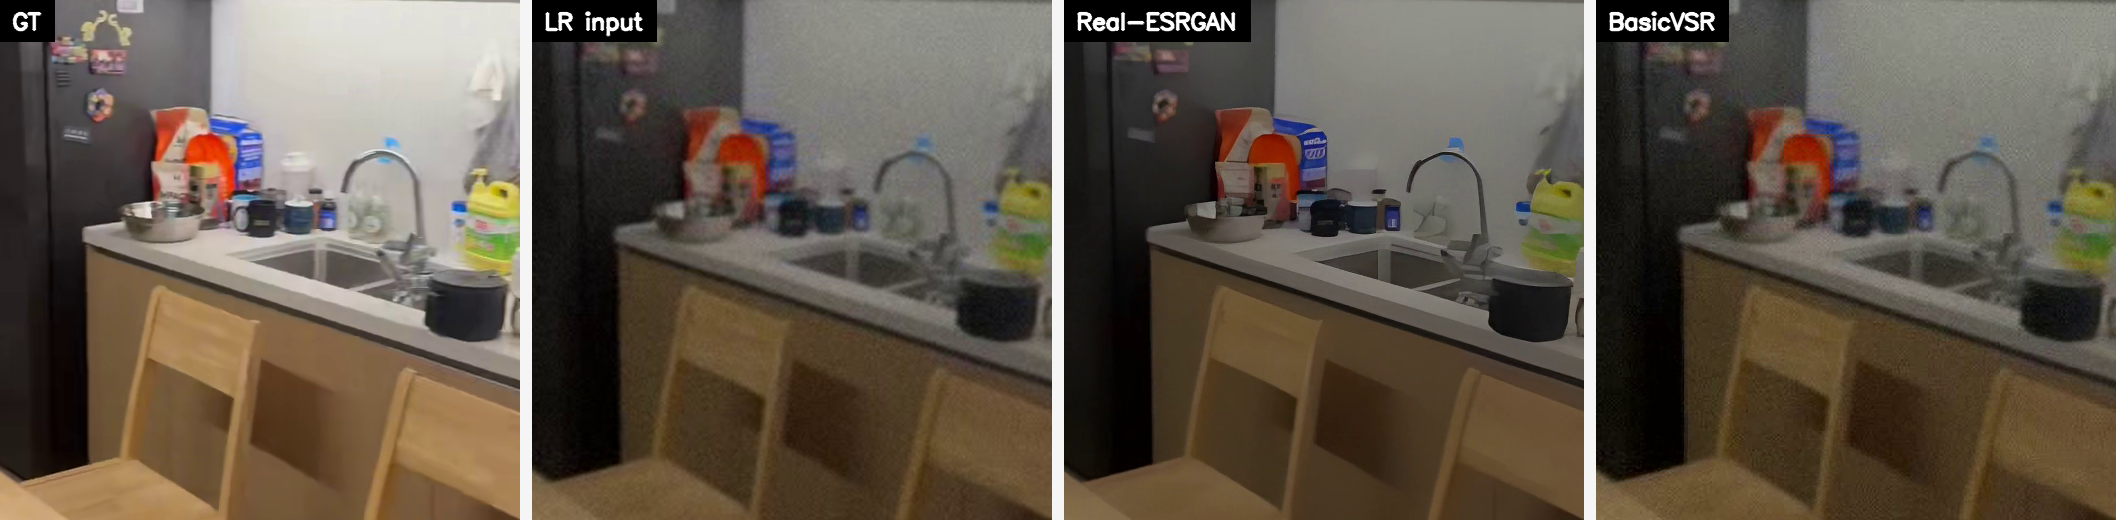
\includegraphics[width=\linewidth]{../../output/figures/wild_realesrgan_basicvsr/wild_frame_0080_zoom.png}
    \caption{Zoomed comparison on the wild video. Zoom-in patches are useful for discussing edge sharpness, texture recovery, and hallucinated details.}
    \label{fig:wild_zoom}
\end{figure}

Figure~\ref{fig:part3_flow} illustrates the flow-stabilized Part 3 output. The main advantage is not always visible from a single frame; it is more apparent when watching videos because small frame-to-frame texture changes are reduced.

\begin{figure}[t]
    \centering
    % FIGURE: existing Part 3 flow-stabilized panel.
    % Existing path: output/figures/wild_real_lr_part3_flow/wild_frame_0080_full.png
    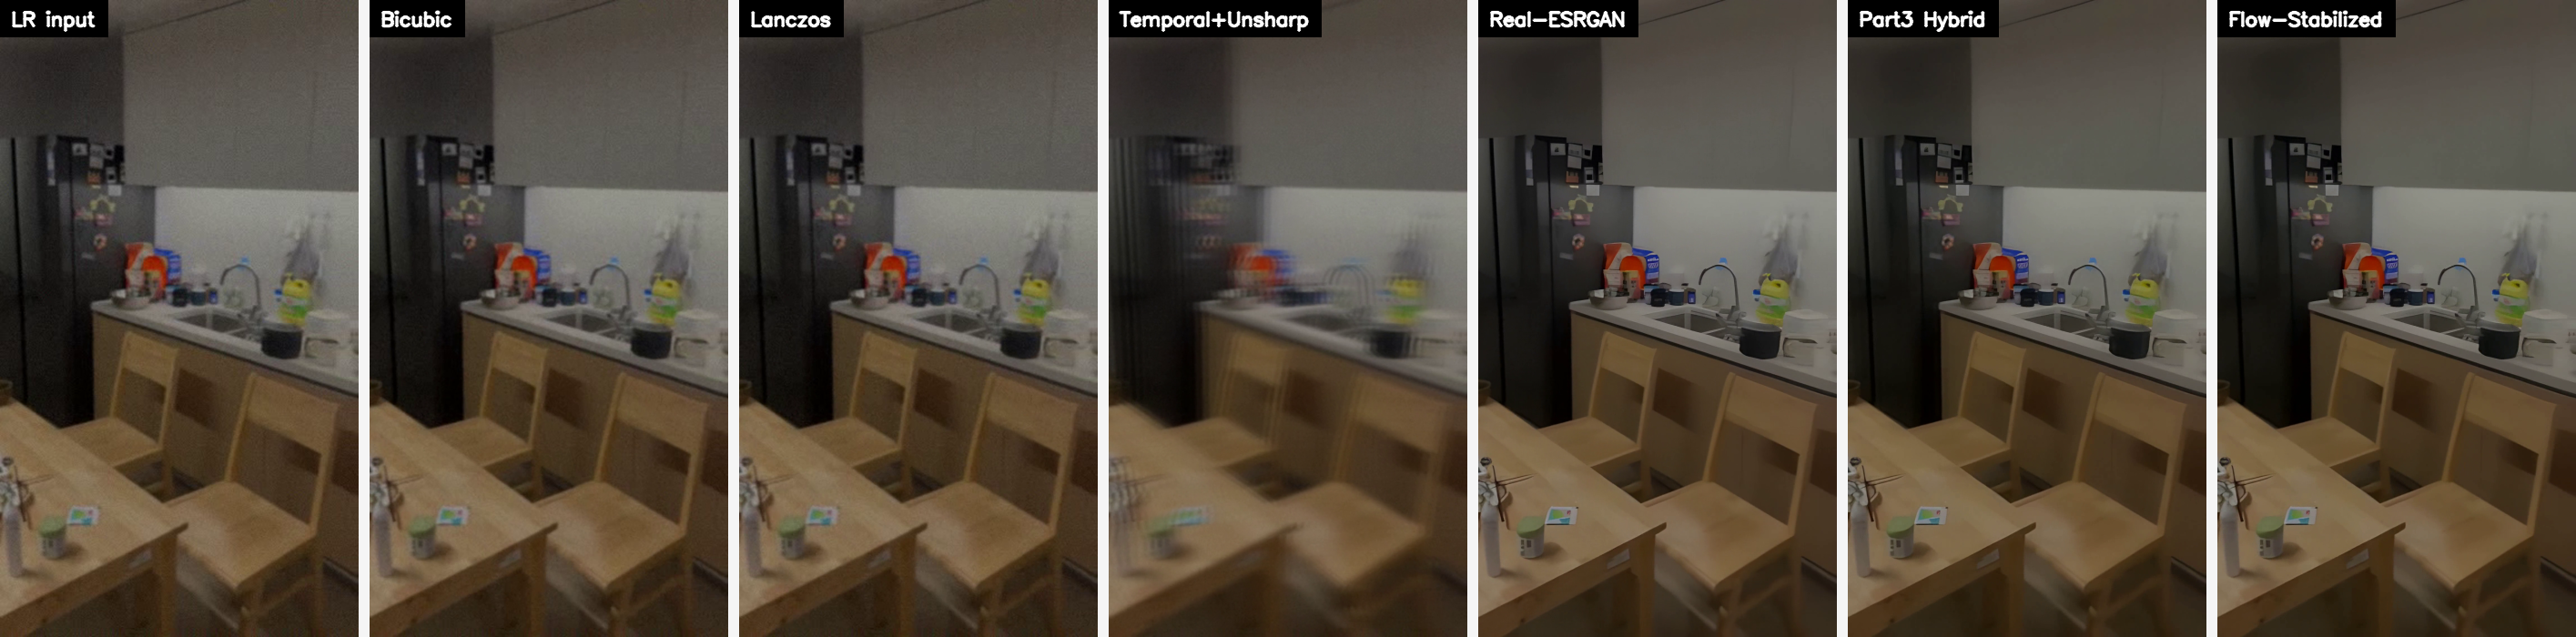
\includegraphics[width=\linewidth]{../../output/figures/wild_real_lr_part3_flow/wild_frame_0080_full.png}
    \caption{Part 3 flow-stabilized output. The method is designed to reduce temporal flicker in the enhanced video.}
    \label{fig:part3_flow}
\end{figure}

\section{Discussion}

The experiments reveal three practical lessons. First, PSNR and perceptual quality do not always agree. Bicubic can obtain high PSNR on aligned synthetic data but remains blurry. Second, pretrained models have degradation assumptions. BasicVSR is powerful, but it may underperform when the input degradations differ from the expected training setting. Third, generative refinement must be used carefully. It can produce plausible textures, but hallucinated details and temporal inconsistency are serious risks for video.

For the final submitted videos, we therefore keep Real-ESRGAN as the strongest direct perceptual baseline and use optical-flow stabilization as the most practical Part 3 refinement. We still report Directions A, C, and D because they demonstrate meaningful exploration and explain why more complex generative systems were not selected as the default final pipeline.

\section{Conclusion}

We completed all three mandatory parts of the project and added an optional Vimeo-90K benchmark subset for stronger evaluation. Part 1 provides reproducible baselines and validates the video pipeline. Part 2 shows that Real-ESRGAN gives strong perceptual quality, while BasicVSR provides an important video-specific comparison. Part 3 explores multiple refinement strategies and identifies optical-flow stabilization as the best practical extension under our time and compute constraints. The main limitations are the lack of HR ground truth for all mandatory/wild videos, the sensitivity of pretrained models to degradation mismatch, and the temporal instability risk of generative refinement. Future work should evaluate larger REDS/Vimeo-90K subsets, fine-tune video-specific restoration models, and incorporate stronger temporal perceptual losses during training.

{\small
\bibliographystyle{ieeenat_fullname}
\bibliography{references}
}

\end{document}


